\documentclass[hyperref={colorlinks = true,linkcolor = blue, citecolor=blue,urlcolor=blue}]{beamer}  
\usetheme{default}

\usepackage{amsthm,amsmath,amssymb}
\usepackage{dsfont}
\usepackage{graphicx}
\usepackage{natbib}
\usepackage[space]{grffile}


\title{The Impact of Natural Disasters on Education: \\ Evidence from Standardized Testing}
\author{Gregor Steiner}
\date{June 10, 2022}

\begin{document}
	
	
	
\begin{frame}[plain]
    \maketitle
\end{frame}

\begin{frame}{Goal}
	I attempt to answer two questions:
	\begin{itemize}
		\item \textbf{What is the causal effect of natural disasters on academic achievement as measured by standardized test scores?}
		\item What is the role of federal disaster assistance? Which counties apply for assistance?
	\end{itemize}
\end{frame}

\begin{frame}{Data}
	\begin{itemize}
		\item \textbf{Natural disasters}:
		\begin{itemize}
			\item Federal Emergency Management Agency (FEMA) declarations 
			\item Storms from the National Weather Service (NWS)
			\item Work in progress: Data on heat waves
		\end{itemize}
		\item \textbf{Public Assistance applications and payments} from FEMA
		\item \textbf{Standardized testing outcomes} from the Stanford Education Data Archive (SEDA):
		\begin{itemize}
			\item Cohort standardized average scores by county in Mathematics \& Reading Language Arts
			\item Grades 3 through 8 for schoolyears 2008/2009 to 2017/2018
		\end{itemize}
	\end{itemize}
\end{frame}

\begin{frame}{Empirical Strategy}
	\begin{itemize}
		\item Event-study design:
		\begin{align*}
			y_{i, t, g} = \beta_{-5}  D_{i, t-5} + \sum_{l = -4, l \neq -1}^{8} \beta_l D_{i, t-l} + \alpha_i + \lambda_t + \zeta_g + \varepsilon_{i, t, g}
		\end{align*}
		\item Heterogenous treatment effects $\implies$ simple TWFE is inadequate \citep{deChaisemartin_2020, Sun_2021}
		\item Solution: Interaction-Weighted Estimator (IW) by \cite{Sun_2021}
		\item Identifying Assumptions: Parallel Trends \& No Anticipatory Behavior
		\item IW consistently estimates a weighted average of cohort average treatment effects on the treated (CATT)
	\end{itemize}
\end{frame}

\begin{frame}{Main Results: FEMA}
	\begin{figure}[!h]
		\centering
		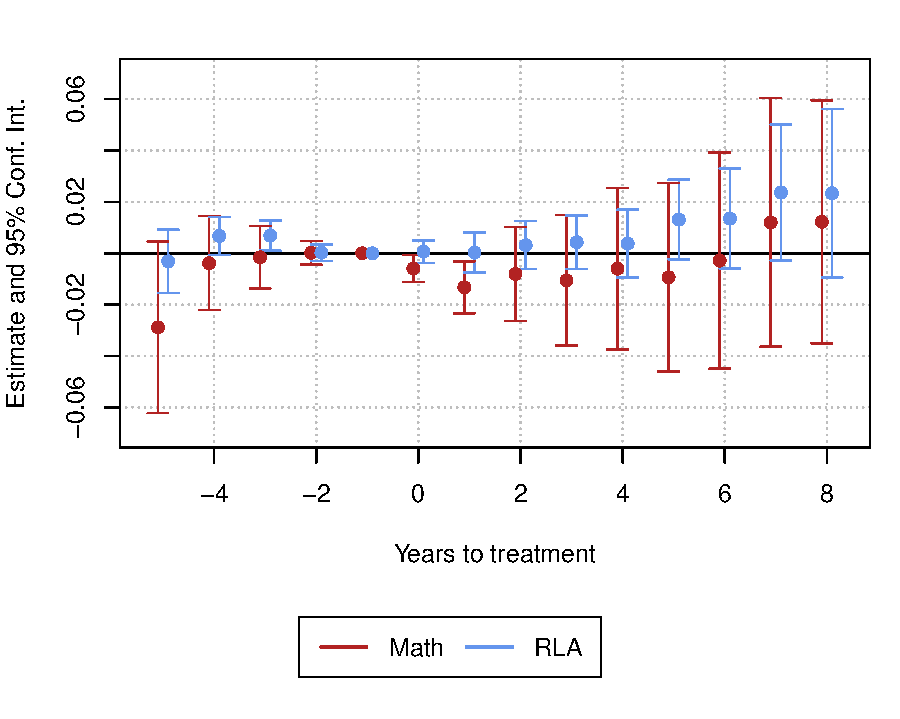
\includegraphics[scale=0.6]{"../Code & Data/ResultsPlotPresentation.pdf"}
		\caption{Dynamic Treatment effects in relative time: FEMA disaster data}
		\label{ResultsPlot}
	\end{figure}
\end{frame}


\begin{frame}{Main Results: Subgroups, FEMA}
	\begin{figure}[!h]
		\centering
		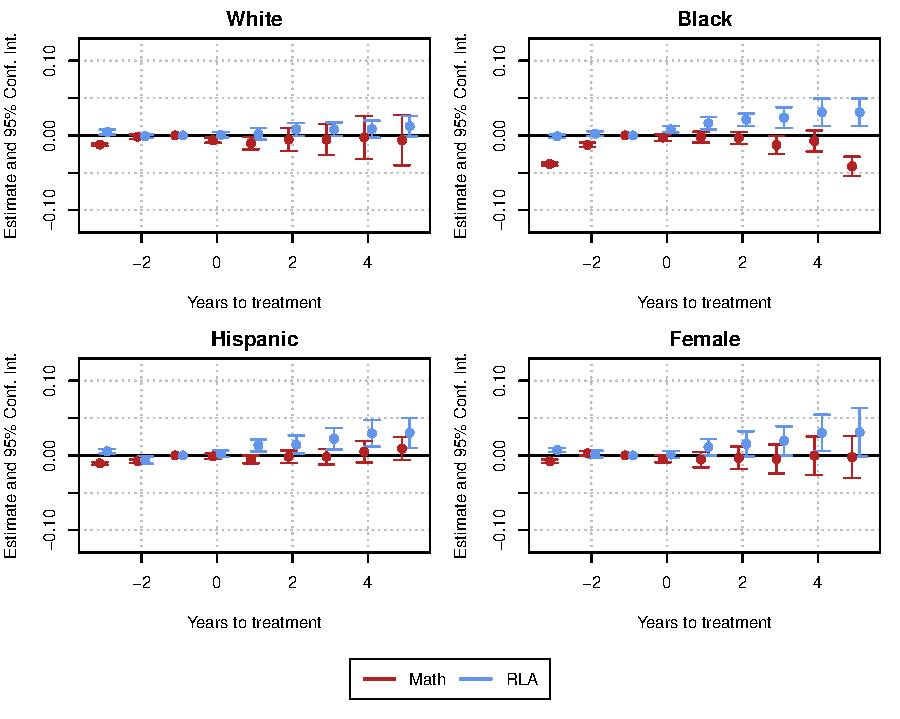
\includegraphics[scale=0.6]{"../Code & Data/ResultsPlotPresentationSubgroups.pdf"}
		\caption{Dynamic Treatment effects in relative time: FEMA disaster data}
		\label{ResultsPlot}
	\end{figure}
\end{frame}


\begin{frame}{Main Results: Storms}
	\begin{figure}[!h]
		\centering
		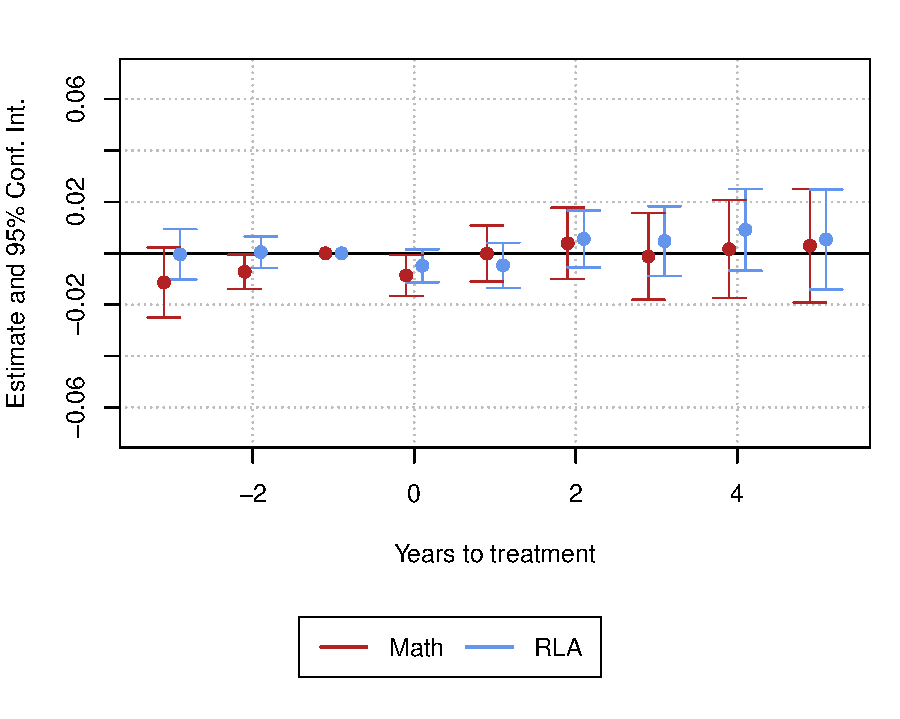
\includegraphics[scale=0.6]{"../Code & Data/ResultsPlotStormsPresentation.pdf"}
		\caption{Dynamic Treatment effects in relative time: FEMA disaster data}
		\label{ResultsPlot}
	\end{figure}
\end{frame}


\begin{frame}{Main Results: Subgroups, Storms}
	\begin{figure}[!h]
		\centering
		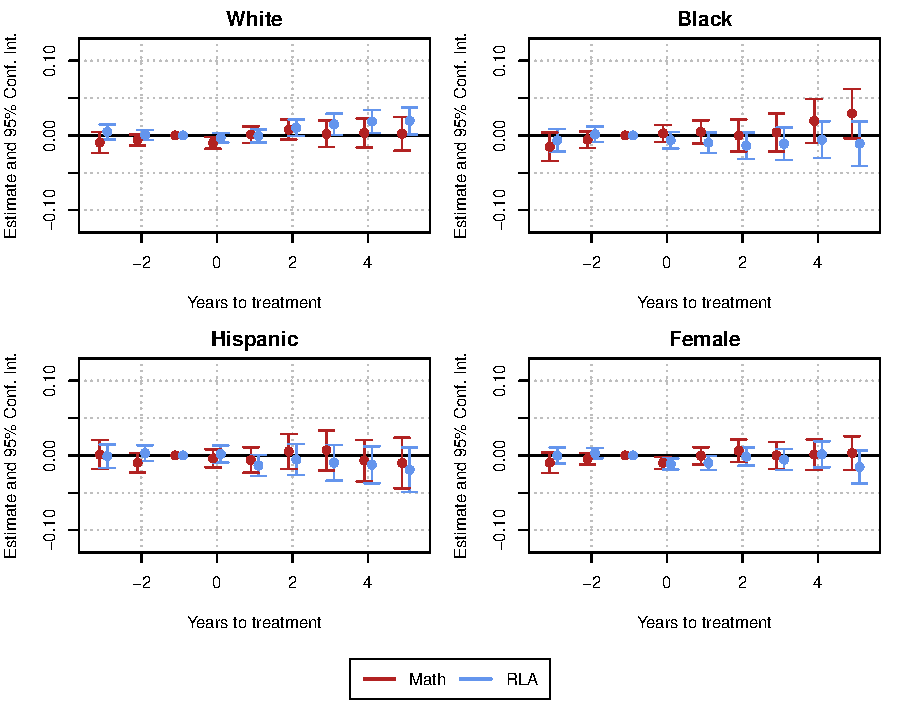
\includegraphics[scale=0.6]{"../Code & Data/ResultsPlotStormsPresentationSubgroups.pdf"}
		\caption{Dynamic Treatment effects in relative time: FEMA disaster data}
		\label{ResultsPlot}
	\end{figure}
\end{frame}


\begin{frame}{Composition Changes?}
	
	\begin{figure}[!h]
		\centering
		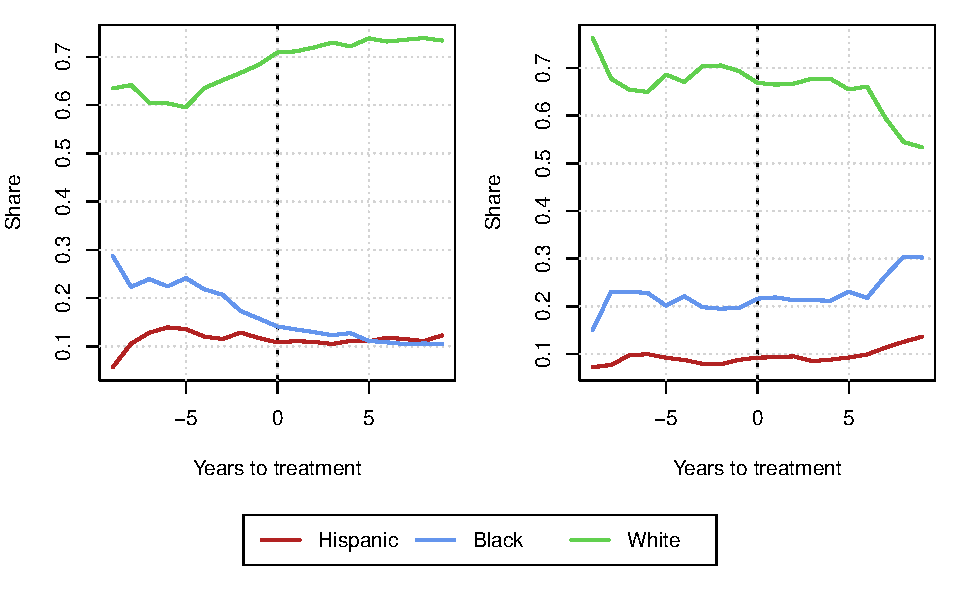
\includegraphics[scale=0.6]{"../Code & Data/EthnicComposition.pdf"}
		\caption{Aggregated ethnic shares by treatment timing based on FEMA disasters (left) and on NWS storms (right)}
		\label{EthnicComposition}
	\end{figure}
\end{frame}






\begin{frame}{References}
	% bibliography
	\bibliographystyle{apalike}
	\bibliography{references}
\end{frame}




\end{document}
